

\colorlet{outlinecolor}{green}

\colorlet{headercolor}{outlinecolor}
\colorlet{rowcolor1}{outlinecolor!70}
\colorlet{rowcolor2}{outlinecolor!50}

\begin{tikzpicture}
	\node [mybox, fill=boxcolor, draw=outlinecolor] (box){%
		\begin{minipage}{0.3\textwidth}
			\vspace{0.1cm}
			\underline{Installation}: Depends on your OS.
			\begin{itemize}
				\item \textit{MacOS.} Normally, it's pre-installed. Otherwise, use command line developer tools to install it.
				\item \textit{WindowsOS.} Install the open source \href{https://gitforwindows.org}{Git for Windows Project}. Make sure to execute your Git commands from the \textcolor{outlinecolor}{Git Bash}.
			\end{itemize}
			
			\underline{Configure \& initialize}: You need to tell Git who you are and where the remote repository hosting platform is.
			\vspace{-2mm}
			\begin{center}
				\textcolor{background}{
					\begin{tabularx}{\textwidth}{>{\columncolor{rowcolor1}}X|>{\columncolor{rowcolor2}}p{4cm}}
						\arrayrulecolor{boxcolor} % Table line color
						\rowcolor{headercolor} % Header row color
						\multicolumn{1}{c|}{\centering \textbf{Git Command}} & \multicolumn{1}{c}{\centering \textbf{Description}} \\ % Center the header text
						\hline % Add a horizontal line below the header row
						\rowcolor{rowcolor1} \tablebash{git config --global user.name "bellanich"} & Set your global username \\
						\rowcolor{rowcolor2} % Color of the second row
						\tablebash{git config --global user.email "youremail@gmail.com"} & Set your global email \\
						\rowcolor{rowcolor1} \tablebash{git config --global --list} & Check your global configs \\
					\end{tabularx}
				}
			\end{center}
			
			\underline{Initialize your project}: Here's how to start a new Git project.
			\vspace{-2mm}
			\begin{center}
				\textcolor{background}{
					\begin{tabularx}{\textwidth}{>{\columncolor{rowcolor1}}X|>{\columncolor{rowcolor2}}p{4cm}}
						\arrayrulecolor{boxcolor} % Table line color
						\rowcolor{headercolor} % Header row color
						\multicolumn{1}{c|}{\centering \textbf{Git Command}} & \multicolumn{1}{c}{\centering \textbf{Description}} \\ % Center the header text
						\hline % Add a horizontal line below the header row
						\rowcolor{rowcolor1} \tablebash{git init my-project-name} & Initialize a new empty Git repository \\
						\rowcolor{rowcolor2} % Color of the second row
						\tablebash{git init} & Convert an existing dir into a Git project \\
						\rowcolor{rowcolor1} \tablebash{git clone git-project-url} & Initialize from your code hosting platform of choice \\
						\rowcolor{rowcolor2} \tablebash{git remote add origin git-project-url} & Add a remote reference to your local repository  \\
						\rowcolor{rowcolor1} \tablebash{git push origin main} & Force push to main branch (only do for initialization)  \\
					\end{tabularx}
				}
			\end{center}

			
%			\begin{minipage}{\textwidth}
%				\centering
%%				\vspace{-2mm}
%				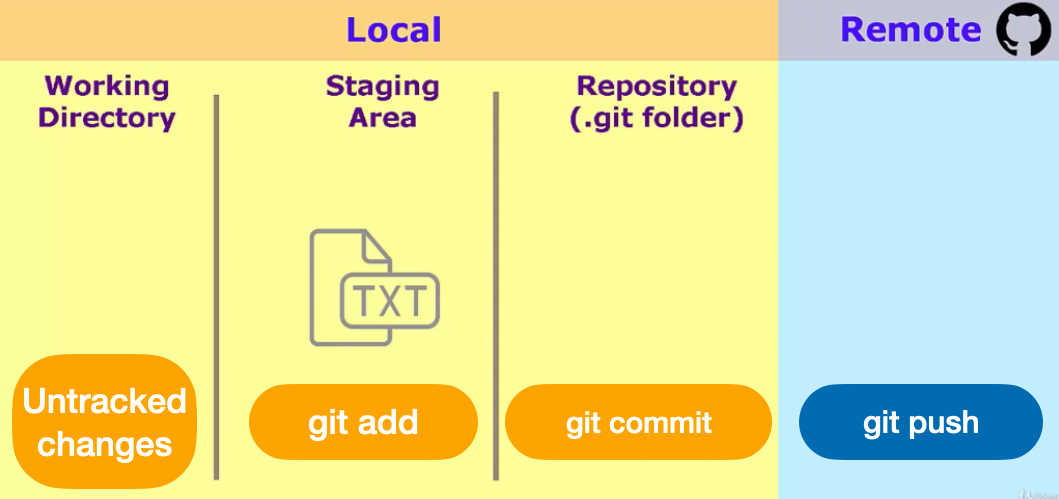
\includegraphics[width=0.5\textwidth]{images/git_stages.png}
%				\vspace{-2mm}
%				\captionof{figure}{Git states and associated commands. \href{https://www.udemy.com/course/git-complete/}{ \faLink{}  Source}}
%			\end{minipage}
			
		\end{minipage}
	};
	\node[fancytitle, right=10pt, fill=outlinecolor, text=background, draw=outlinecolor, rounded corners] at (box.north west) {Quick Start};
\end{tikzpicture}
